%%%%%%%%%%%%%%%%%%%%%%%%%%%%%%%%%%%%%%%%%%%%%%%%%%%%%%%%%%%%%%%%%%%%%%%%%%%%%%%%
\chapter{Детали реализации}
%%%%%%%%%%%%%%%%%%%%%%%%%%%%%%%%%%%%%%%%%%%%%%%%%%%%%%%%%%%%%%%%%%%%%%%%%%%%%%%%

Данный раздел посвящен описанию реализации механизма классов типов. Сначала будет приведен краткий обзор внутреннего устройства компилятора языка программирования Kotlin, после чего будут описаны детали реализации частей разработанного механизма. Для удобства разработки процесс непосредственной реализации механизма классов типов был разделен на две части: реализацию прототипа, обеспечивающего основную функциональность, и последующие его модификации. 

Весь разработанный в рамках данной работы программный код может быть найден в публичном репозитории, расположенном по адресу \url{https://github.com/JohnKhandygo/kotlin}. Данный проект является точным клоном ветки \code{master} проекта компилятора языка программирования Kotlin, датированный $31.01.2017$ (номер ревизии \code{81dc30fe5e1d94d20a992bf0bf0836f360ede3eb}), со всеми описанными далее модификациями. 

Также стоит отметить, что все приведенные далее диаграммы классов используются для наглядности и отображают только ту часть структуры классов, которая релевантна в контексте рассматриваемых деталей реализации. Таким образом, строго говоря, данные диаграммы не могут считаться корректными, поскольку не соответствуют описаниям классов в исходном коде компилятора Kotlin в полной мере. Тем не менее, все представленные на диаграммах классы и методы (с точностью до списка аргументов) действительно присутствуют в исходном коде компилятора. С особенностями графической нотации использованных диаграмм можно ознакомиться на электронном ресурсе, расположенному по адресу \url{http://plantuml.com/class-diagram}. Также в рамках данного раздела для простоты объединим программные сущности, соответствующие объявлениям класса, интерфейса, перечисления (enum) и объекта единым термином <<класс>>.  

\section{Внутреннее устройство компилятора языка программирования Kotlin}

Работу компилятора языка программирования Kotlin можно разделить на два этапа: анализ исходных текстов программы и генерация байт-кода. 

\begin{figure}[htbp]
    \centering
    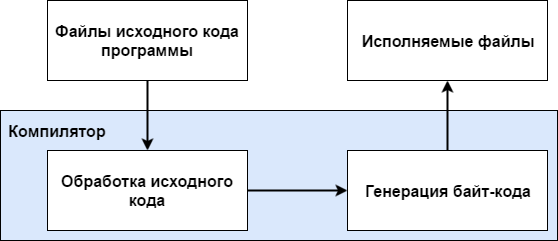
\includegraphics[width=\textwidth]{resources/06/01_compiler_scheme.png}
    \caption{Этапы работы компилятора языка программирования Kotlin}
    \label{fig:compiler-scheme}
\end{figure}

На первом этапе сначала происходит синтаксический разбор текста исходного кода программы, в результате чего формируется абстрактное синтаксическое дерево (abstract syntax tree --- AST), описывающие программу. Затем на основе полученной модели строится абстрактный семантический граф программы (abstract semantic graph --- ASG) который содержит уже не только синтаксическую, но также и семантическую информацию о структуре программы. После построения ASG-модели происходит преобразование ее в набор \emph{дескрипторов}, с которыми удобнее работать на стадии генерации байт-кода. Не все дескрипторы должны предоставлять какую-либо синтаксическую информацию, что позволяет иметь синтетические программные сущности, которые не представлены в исходном коде программы в явном виде. Основное отличие дескрипторов от элементов абстрактного семантического графа заключается в том, что дескрипторы связаны общей системой типов, которая строится по мере анализа программы. Таким образом, именно на этапе анализа программы происходит вычисление всех типов и проверяется корректность их использования. 

Одним из центральных элементов всего процесса компиляции является экземпляр класса \code{BindingTrace}. Во-первых, интерфейс \code{BindingTrace} расширяет интерфейс \code{DiagnosticSink}, который предоставляет методы по сбору диагностических сообщений, что позволяет организовать обратную связь с пользователем. Во-вторых, \code{BindingTrace} позволяет сохранять любую информацию на стадии анализа для дальнейшего ее использования на этапе генерации байт-кода. Хранение информации организовано в виде пар <<ключ-значение>>, где ключ состоит из двух частей: идентификатора среза данных (который также хранит информацию о типах второй части ключа и значения) и обычного ключа, как он понимается в структуре данных <<ассоциативный массив>>. Большинство идентификаторов срезов данных объявлены в интерфейсе \code{BindingContext}, который также предоставляет некоторые операции по работе со срезами данных и сбору диагностических сообщений. Основным отличие \code{BindingContext} от \code{BindingTrace} заключается в том, что, в случае использования первого, данные доступны только для чтения, в то время как в \code{BindingTrace} также заложена возможность записи данных. 

\begin{figure}[htbp]
    \centering
    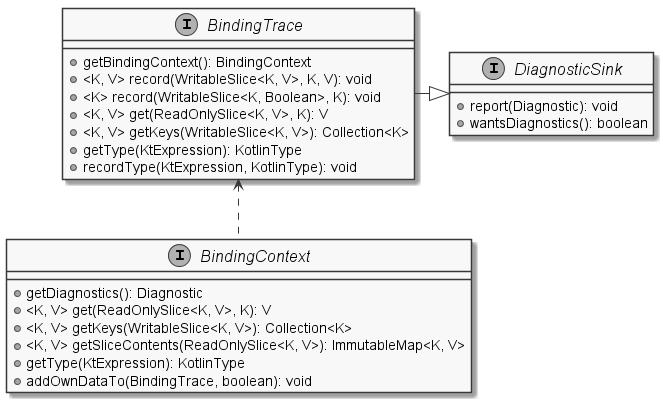
\includegraphics[width=\textwidth]{resources/06/04_binding_context.png}
    \caption{Структура интерфейса \smallcode{BindingTrace}}
    \label{fig:binding-trace-scheme}
\end{figure}

Описание \code{BindingContext} насчитывает порядка шестидесяти объявлений идентификаторов срезов данных. Большинство из них описывают срезы, которые хранят соответствие определений программных сущностей в исходном коде и дескрипторов, однако есть и такие, которые предназначены для хранения информации о типах, потоке данных, областях видимости и т.д. 

\begin{figure}[htbp]
    \centering
    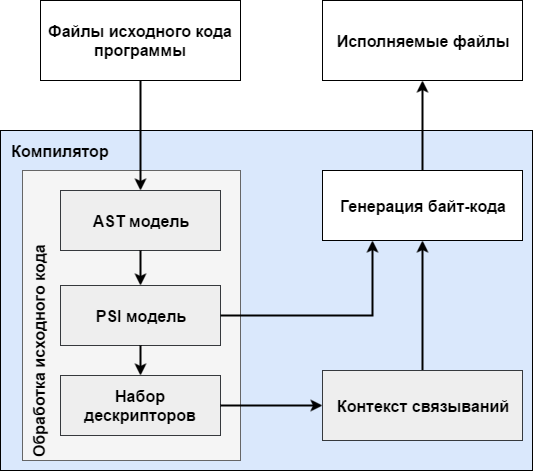
\includegraphics[width=\textwidth]{resources/06/04_compiler_flow_diagram.png}
    \caption{Этапы преобразования языковых конструкций компилятором языка программирования Kotlin}
    \label{fig:binding-trace-scheme}
\end{figure}

После анализа файлов исходного кода в случае, если не было выявлено каких-либо критических ошибок, начинается этап генерации байт-кода. Данный процесс организован последовательно для всех компилируемых файлов. В пределах конкретного файла объявляется следующий порядок обработки элементов: сначала генерируется байт-код для классов, объявленных в данном файле, а затем для всех других определений, которые встречаются в файле (функции, свойства и т.д.). Одним из основных классов здесь является \code{MemberCodegen}: именно в нем определяются базовые методы, отвечающие за генерацию членов классов, а также порядок обработки самого класса. 

\begin{figure}[htbp]
    \centering
    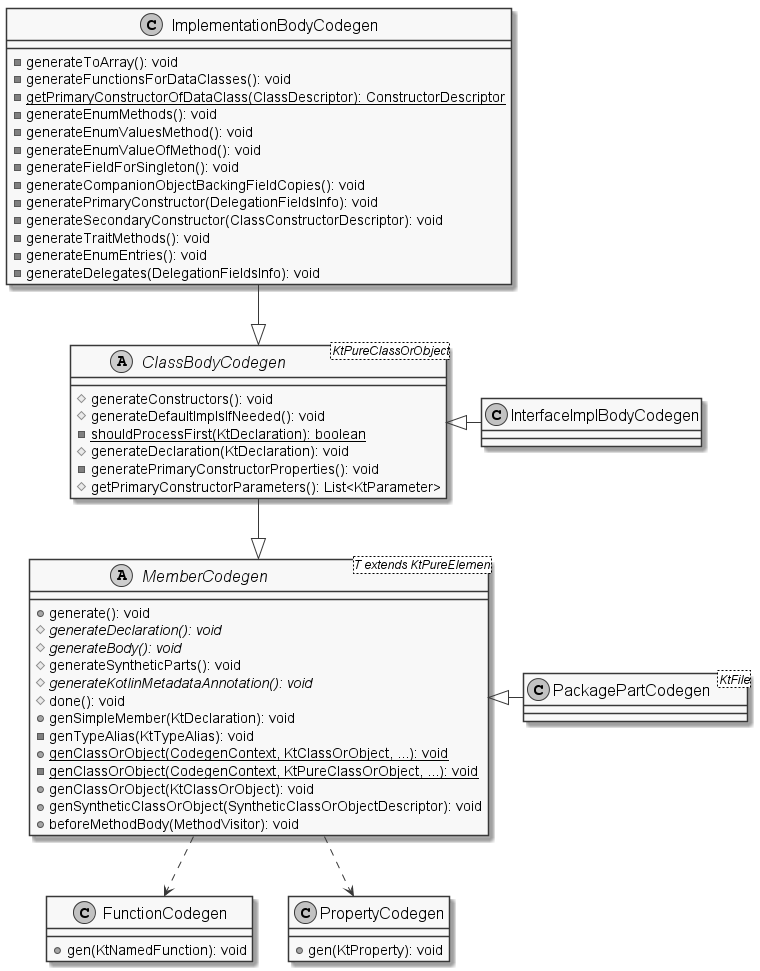
\includegraphics[width=\textwidth]{resources/06/06_member_codegen.png}
    \caption{Структура интерфейса \smallcode{MemberCodegen}}
    \label{fig:binding-trace-scheme}
\end{figure}

Порядок определяется вне зависимости от того, является ли обрабатываемая языковая конструкция классом, интерфейсом или объектом, следующим образом:
\begin{enumerate}
    \item Генерация объявления.
    \item Генерация тела. На данном этапе генерируется байт-код для всех определений, объявленных внутри рассматриваемого класса. Это могут быть как свойства и функции, так и другие классы. В случае, если на этом шаге встречается класс, порядок его обработки также соответствует настоящему списку. 
    \item Генерация синтетических частей. Под синтетическими частями здесь понимается часть функциональности класса, которая абсолютно корректна с точки зрения использования в пользовательском коде, однако не объявляется нигде в исходном коде программы. Сюда, например, относятся специальные функции \code{values} и \code{valueOf}, относящиеся к перечислениям.
\end{enumerate}
Для всякого типа генерируемого определения в компиляторе представлена подходящая реализация \code{MemberCodegen}, в которой определяется каким именно образом будут обрабатываться объявление, тело и синтетические части класса. Свойства и функции, в свою очередь, с точки зрения пользователя \code{MemberCodegen} генерируются для всех классов одинаково.

\section{Разработка прототипа механизма классов типов}

На этапе разработки прототипа приоритетной была поставлена задача реализации и интеграции всех алгоритмов, необходимых для обеспечения существенной части функциональности механизма классов типов. Тем не менее, разрабатываемый прототип должен удовлетворять всем требованиям, представленным в разделе~\ref{sct:problem-constraints}. Такой подход позволяет получить рабочую версию компилятора, которая допускает использование классов типов, однако, возможно, обладает некоторыми недостатками, касающимися в основном выразительной части разработанного механизма. 

Сначала зафиксируем форму представления всех элементов, необходимых для использования классов типов. Возьмем за основу семантику, введенную в разделе~\ref{sct:problem-semantic}, и упростим ее. Прежде всего перечислим основные возможности, которые необходимо предоставить пользователю для полноценного использования классов типов:
\begin{itemize}    
    \item Объявить класс типов.
    \item Объявить экземпляр класса типов.
    \item Объявить принадлежность произвольной типовой переменной функции некоторому классу типов.
    \item Вызвать произвольную функцию, принадлежащую экземпляру класса типов для типовой переменной с соответствующим ограничением.   
\end{itemize}
В соответствии с введенной ранее семантикой предусматривается два способа объявления ограничений на принадлежность типовой переменной классу типов: неявно через определение аргумента, играющего роль словаря функций класса типов, и посредством объявления типовой переменной специального вида. Реализация второго подхода на данном этапе представляется достаточно сложной с точки зрения реализации, поскольку требует разработки дополнительного механизма, предоставляющего доступ к функциям используемого словаря. По этой причине на этапе разработки прототипа механизма классов типов было решено ограничиться рассмотрением только лишь первого подхода, который позволяет использовать словарь функций класса типов в явном виде в теле функций. Таким образом, для реализации прототипа механизма класса типов достаточно модифицировать компилятор таким образом, чтобы:
\begin{itemize}
    \item Всякий раз, когда встречается аргумент, помеченный аннотацией \code{@TypeClassDisctionary} и тип которого соответствует классу типов, организуется поиск подходящего экземпляра класса типов с учетом доступной информации о значениях типовых переменных. Если подходящий экземпляр не был найден, генерируется диагностическое сообщение об ошибке. В противном случае результат поиска сохраняется.
    \item Всякий раз при обработке вызова функции список параметров вызова формируется с учетом дополнительной информации об уже найденных для данного вызова экземплярах классов типов. Если при этом какой-то из аргументов, помеченных аннотацией \code{@TypeClassDisctionary}, указан в рассматриваемой точке вызова в явном виде, генерируется диагностическое сообщение об ошибке.
\end{itemize}
Таким образом, на уровне представления в исходном коде программы предлагаемый подход аналогичен шаблону проектирования <<класс типов>> в языке программирования Scala с той лишь только разницей, что здесь запрещается явное указание аргументов-словарей в точке вызова всякой функции. 

Единственный вопрос, который до сих пор не был рассмотрен, касается стратегии создания словаря функций класса типов перед его передачей непосредственно в точку вызова. Понятно, что в точке вызова функции, использующей классы типов, при применении рассматриваемого подхода не представляется возможным указать аргументы, которые необходимо передать в конструктор соответствующего экземпляра класса типов. Таким образом, на этапе подстановки аргументов в вызов такой функции, необходимо либо уже иметь экземпляр словаря функций классов типов, либо наперед знать о конкретной функции, которая способна такой экземпляр предоставить и которая при этом не принимает аргументов. В дальнейшем для удобства закрепим за такими функциями термин <<\emph{функция-поставщик}>>. В случае использования функции-поставщика сразу же возникает вопрос о сохранении состояния используемого экземпляра класса типов как объекта. Если состояние экземпляра класса типов изменяется в процессе работы, необходимо определить, в какой области его использования такой экземпляр должен быть представлен в единственном виде. Даже если доступ к экземпляру класса типов осуществляется через уже готовую ссылку (фактически, посредством переменной), необходимо среди всех подходящих ссылок выбрать правильную.

Заметим, что наличие более чем одного источника, способного предоставлять словари функций классов типов, предполагает наличие некоторого механизма, который будет выбирать единственный источник. Такой механизм, очевидно, с точки зрения функциональности имеет много общего с механизмом неявных определений, представленном в языке программирования Scala. Напомним, что именно допущение о наличии более чем одного подходящего неявного определения в языке Scala может существенно затруднить или исказить понимание исходного кода программы с точки зрения стороннего пользователя, поскольку задача вычисления неявного определения, используемого в точке вызова произвольной функции, в общем случае является слишком сложной даже для специализированных средств разработки. Кроме того, допущение о наличии более чем одного источника экземпляров классов типов в разрабатываемом механизме способно неявным образом нарушить требование об уникальности экземпляра классов типов даже в случае, когда источник экземпляра класса типов указывается явно в точке вызова. Это становится возможным благодаря тому, как устроена работа с \emph{вариантными} (\emph{variance}) типами в языке программирования Kotlin. Рассмотрим пример, представленный в листинге~\ref{lst:single-instance-violation}. Аннотация \code{@TypeClassSupplier} используется в данном примере для выделения объявлений (свойств, функций, классов специального вида и т.д.), которые тем или иным способом (посредством вызова или обращения, например) способны предоставлять словарь класса типов.  

\lstinputlisting[
    label={lst:single-instance-violation},
    caption={Пример кода, допускающего нарушение требования о единственности экземпляра класса типов},
    style={kotlin}
]
{resources/06/09_single_instance_violation}

Таким образом, в примере, представленном в листинге~\ref{lst:single-instance-violation}, существует два источника, способных предоставить экземпляр класса типов \code{Default} для типа \code{Number}. Пусть существуют две точки вызова произвольных функций (возможно, одинаковых), каждая из которых использует класс типов \code{Default}. Пусть также в одной из таких точек вызова в качестве источника экземпляра класса типов был выбран объект \lstinlint{NumberDefault}, а в другом --- функция \code{getDefaultForNumber}. Тогда в две эти точки вызова будут подставлены разные реализации интерфейса \code{Default}, каждая из которых является экземпляром класса типов \code{Default} для типа \code{Number}. Здесь можно сказать, что уже из самих объявлений экземпляров классов типов следует нарушение требования единственности на основании того, что экземпляр класса типов \code{Default} для типа \code{Number} с точки зрения системы типов может быть использован вместо экземпляра для типа \code{Double}. Это утверждение легко опровергнуть, поскольку, несмотря на наличие более чем одного подходящего экземпляра, в такой ситуации компилятор может быть запрограммирован таким образом, чтобы выбор был сделан в сторону наиболее точного по типу экземпляра. В свою очередь, в примере, представленном в листинге~\ref{lst:single-instance-violation}, реализация такого подхода не представляется возможным.   

Учитывая приведенные выше доводы, было решено ввести ограничение на уникальность источника, предоставляющего экземпляры словарей функций классов типов. Вопрос о том, какой вид источников предпочтителен, остается открытым. С одной стороны, использование функций-поставщиков представляется более гибким, поскольку позволяет отделить конфигурацию объектов от их использования (что, строго говоря, является одним из основных архитектурных принципов в объектно-ориентированном программировании). Альтернативный подход заключается в том, чтобы для каждого экземпляра класса типов была определенная единственная переменная, которая используется всюду для доступа к соответствующему экземпляру класса типов. Такой подход равносилен использованию шаблона проектирования <<одиночка>> (singleton)~\cite[стр.~177--189]{Martin03} по отношению ко всем экземплярам классов типов. Использование второй стратегии, конечно, обязывает пользователя разрабатывать экземпляры классов типов таким образом, чтобы они были безопасны для использования несколькими потоками исполнения и, к тому же, быть более осторожным при введении изменяемого состояния объекта, однако, в то же время представляется более простой для реализации. Именно поэтому на этапе разработки прототипа было решено осуществлять доступ к экземплярам классов типов вторым способом. Стоит отметить, что язык программирования Kotlin по умолчанию поддерживает шаблон проектирования <<одиночка>>. Для этого в язык был введен новый для Java вид объявлений --- объекты. Объекты по сути являются классами, для которых компилятор автоматически генерирует и инициализирует статическое поле для хранения единственного экземпляра данного класса. Таким образом, было решено сделать предлагаемый подход более наглядным и еще более простым с точки зрения реализации, ограничив способы определения экземпляров классов типов только лишь объектами. 

\lstinputlisting[
    label={lst:demo-usage-example},
    caption={Пример использования классов типов в прототипе механизма классов типов},
    style={kotlin}
]
{resources/06/08_demo_usage_example}

Также в рамках разработки прототипа механизма классов типов для упрощения задачи были использованы следующие ограничения:
\begin{itemize}
    \item Не учитывается вариантность типовых переменных класса типов.
    \item В качестве экземпляров классов типов рассматриваются только прямые наследники интерфейса, описывающего класса типов.
    \item Не рассматриваются варианты использования экземпляров классов типов, определенных в сторонних библиотеках.
\end{itemize}

\section{Реализация прототипа механизма классов типов}

Процесс обработки объявлений классов типов, их экземпляров и функций, использующих классы типов, в базовой версии разрабатываемого механизма был реализован следующим образом:  
\begin{enumerate}
    \item Каждый раз, когда встречается определение объекта, который является прямым наследником типа, объявление которого помечено аннотацией \code{@TypeClass}, извлекается множество значений типовых переменных, присущих этому типу. Затем дескрипторы этого объекта и объявления его базового типа вместе со значениями всех значимых типовых переменных сохраняются. 
    \item В месте разрешения вызова функции для всякого аргумента, помеченного аннотацией \code{@TypeClassDictionary}, вычисляется его тип с учетом значений типовых переменных, доступных в области видимости рассматриваемого вызова, и все известные типы экземпляров классов типов проверяются на соответствие этому вычисленному типу. После этого извлекается определение объекта, соответствующее найденному типу экземпляра класса типов. Найденное таким образом объявление, вызов и соответствующий аргумент, сохраняются. В случае, если подходящего экземпляра класса типов не было найдено, генерируется сообщение об ошибке, а значение рассматриваемого аргумента принимается равным \code{null}. 
    \item Перед генерацией аргументов вызова на стеке вместе с объявленными аргументами извлекаются также значения всех неявных параметров, вычисленных для данного вызова. Все аргументы объединяются в единый список в порядке, соответствующем порядку объявления аргументов в определении функции, который в дальнейшем используется по стандартному сценарию.    
\end{enumerate}   
Рассмотрим каждый из этих этапов более подробно. Всякий дескриптор класса владеет информацией о собственном базовом типе (включая значения типовых переменных) и его дескрипторе. Таким образом, первый этап описанного выше процесса теоретически может быть реализован сразу после создания дескриптора класса. Основная логика, связанная с управлением процессом создания дескрипторов, расположена в классе \code{LazyTopDownAnalyzer}. 

\begin{figure}[htbp]
    \centering
    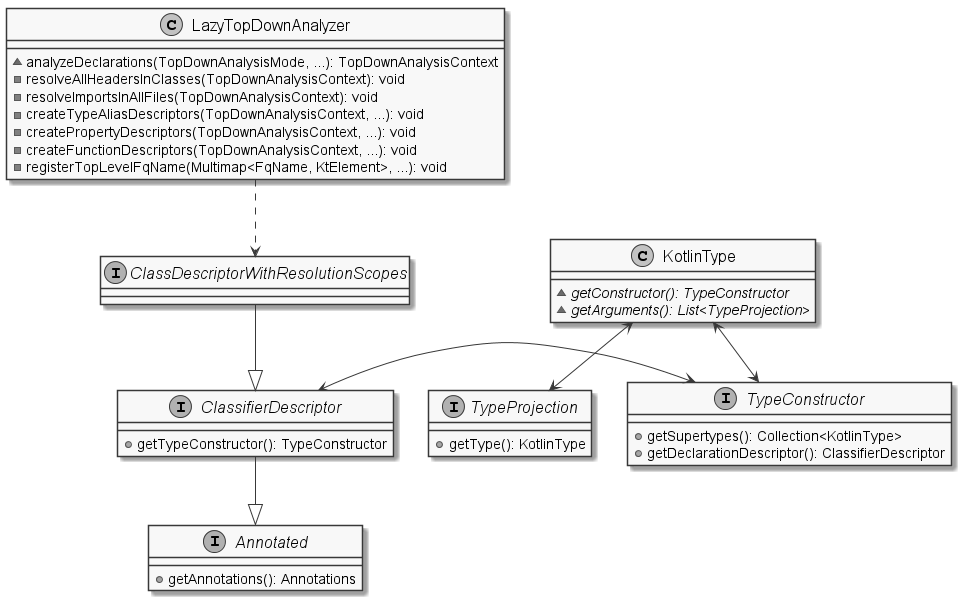
\includegraphics[width=\textwidth]{resources/06/12_class_descriptor.png}
    \caption{Структура класса \smallcode{LazyTopDownAnalyzer}}
    \label{fig:lazy-top-down-analyzer}
\end{figure}

Здесь организован рекурсивный перебор всех деклараций, находящихся в компилируемых файлах. Дескрипторы классов создаются прямо в процессе перебора ленивым образом, в то время как все остальные декларации просто запоминаются и преобразуются в дескрипторы уже после просмотра предоставленных файлов. Стоит обратить внимание на то, что большинство компонент деклараций, соответствующих объявлениям классов в исходном коде программы, также создаются ленивым образом. Ленивые вычисления здесь играют важную роль, поскольку позволяют не только игнорировать порядок обхода файлов компилятором, но к тому же разрешать некоторые циклические зависимости в исходном коде. В некоторых случаях преждевременное обращение к определенным составляющим дескриптора класса может привести к исключению на этапе компиляции. Таким образом, обработку информации об экземплярах классов типов целесообразно проводить уже после того, как все компоненты дескрипторов классов могут быть вычислены. Это становится возможным в самом \code{LazyTopDownAnalyzer} после того, как будет вызван метод \code{resolveAllHeadersInClasses}. Более того, внутри этого метода компоненты всех найденных дескрипторов классов вычисляются и, соответственно, дальнейшие манипуляции с дескрипторами не нарушают неявных контрактов, связанных с ленивыми вычислениями. Хранить информацию об экземплярах классов типов было решено внутри контекста связываний. Такое решение можно объяснить тем, что экземпляр одного из типов \code{BindingTrace} или \code{BindingContext} доступен практически на любом этапе компиляции программы, что позволяет обеспечить доступ к информации о классах типов там, где это будет необходимо. Идентификатор соответствующего среза данных был определен внутри объявления \code{BindingContext} следующим образом:

\begin{lstlisting}[style={wo_caption}]
WritableSlice<
 ClassDescriptor, 
 Map<List<KotlinType>, ClassDescriptor>> 
 TYPECLASS_IMPLEMENTATIONS = Slices.createSimpleSlice();
\end{lstlisting}

Теперь, когда информация о классах типов и их экземплярах сохраняется в контексте связываний, перейдем к рассмотрению процессов обработки и генерации вызовов функций. За генерацию байт-кода вызова функции отвечает класс \code{ExpressionCodegen}. Сам класс реализует интерфейс посетителя в шаблоне проектирования <<посетитель>> (visitor)~\cite[стр.~387--419]{Martin03}, в котором элементами являются декларации. Таким образом, \code{ExpressionCodegen} обрабатывает не только вызовы, но также и все другие существующие виды объявлений. Аргументы вызова извлекаются из экземпляра класса \code{ResolvedCall}, который хранится в специальном  срезе данных в контексте связываний.     

\begin{figure}[htbp]
    \centering
    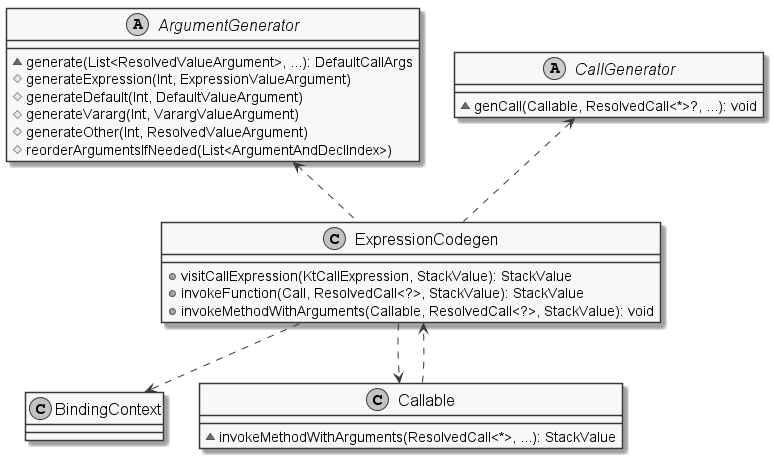
\includegraphics[width=\textwidth]{resources/06/11_expression_codegen.png}
    \caption{Структура класса \smallcode{ResolvedCall}}
    \label{fig:expression-codegen}
\end{figure}

Экземпляры класса \code{ResolvedCall} создаются и сохраняются на этапе поиска функции-кандидата, вызов которой обрабатывается. За формирование списка параметров вызова отвечает класс \code{CandidateResolver}. Опишем наиболее релевантные с точки зрения рассматриваемой задачи этапы обработки аргументов вызовов в порядке их исполнения:
\begin{enumerate}
    %\item Проверка фиктивности дескриптора функции-кандидата. Если дескриптор фиктивный, то никаких дальнейших проверок не производится, при этом считается, что процесс разрешения этого кандидата завершен успешно.  
    %\item Проверка области видимости класса, членом которого является рассматриваемый кандидат. 
    \item В зависимости от режима проверки типов либо происходит сопоставление значений аргументов вызова параметрам рассматриваемой функции-кандидата, либо производится проверка возвращаемого типа функции. В первом случае в экземпляр класса \code{ResolvedCall} добавляется информация о соответствии аргументов функции-кандидата и значениях, указанных в точке вызова, а также для каждого известного аргумента записывается статус, который отражает состояние аргумента в системе типов функции кандидата.  
    %\item Проверка типов ресиверов (receivers) функции.
    \item Если значения типовых переменных указаны явно в точке вызова, то строится соответствующий им подстановщик типов, который затем используется для присвоения значений типовым переменным внутри дескриптора кандидата.
    \item Проверка значений аргументов функции в точке вызова. Если значения типовых переменных указаны явно в точке вызова, то значения аргументов проверяются на соответствие полученной системе типов. В противном случае, типы параметров функции в точке вызова вычисляются, при этом в процессе вычисления типов строится соответствующая им система типов. Вызов в этом случае считается корректным если полученная система типов не имеет противоречий.      
    %\item Проверка того, что рассматриваемая функция-кандидат не является абстрактной. Также проверяются некоторые специальные случаи использования суперклассов.
    %\item Проверка корректности использования вызова в случае, если рассматриваемый кандидат является конструктором псевдонима типов (type alias). 
\end{enumerate}

\begin{figure}[htbp]
    \centering
    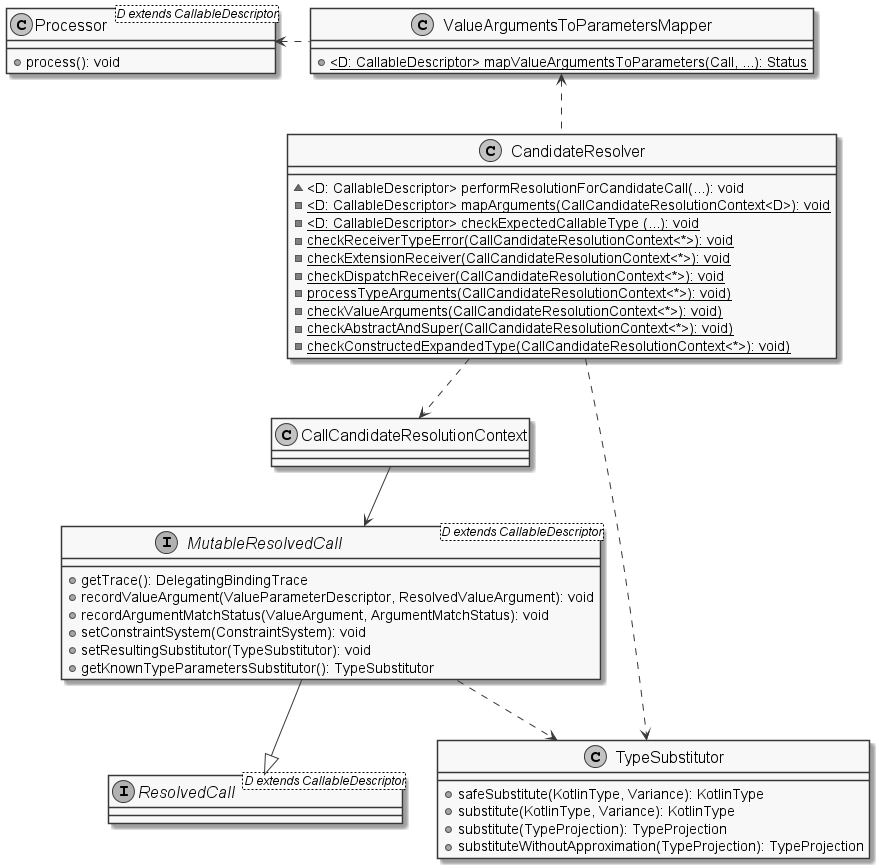
\includegraphics[width=\textwidth]{resources/06/13_candidate_resolver.png}
    \caption{Структура класса \smallcode{CandidateResolver}}
    \label{fig:candidate-resolver}
\end{figure}

Напомним, что в соответствии с предложенным подходом, неявные аргументы не указываются в точке вызова. Таким образом, ошибка компиляции в описанном выше процессе, возникает уже на первом шаге. Для разрешения этой проблемы в процессе обхода аргументов функции-кандидата производится проверка на присутствие аннотации \code{@TypeCLassDictionary}. В случае, если рассматриваемый аргумент помечен такой аннотацией, его значение не извлекается из списка параметров, указанного в точке вызова, но принимается равным выражению \code{null}. Помимо этого, в соответствие такому аргументу ставится специальный статус, который позднее позволит отличить аргументы, значения которых должны быть вычислены компилятором самостоятельно, от тех, которые указываются пользователем. Теперь необходимо определить точку, в которой экземпляр \code{ResolvedCall} получает информацию о значениях типовых переменных. Вся информация, касающаяся данного аспекта вызова содержится в экземпляре класса \code{TypeSubstitutor} (подстановщик типов), обработка которого происходит в методе \code{setResultingSubstitutor} класса \code{ResolvedCall}. В случае, если значения типовых переменных указаны явно в точке вызова, соответствующий подстановщик типов строится и передается на обработку уже на втором этапе описанного выше процесса. В противном случае, подстановщик типов будет построен позже (за это отвечает класс \code{GenericCandidateResolver}), однако обрабатываться он будет таким же образом. В процессе обработки подстановщика типов в \code{ResolvedCall} все известные до этого параметры создаются заново с учетом новой информации о значениях типовых переменных. Кроме того, внутри экземпляра класса \code{ResolvedCall} есть доступ к экземпляру класса \code{BindingTrace}. Таким образом, здесь не представляет большой сложности выбрать подходящий экземпляр класса типов: достаточно извлечь список параметров типа аргумента, играющего роль словаря класса типов, и, используя этот список и дескриптор объявления типа как ключ, запросить все доступные экземпляры класса типа из известного среза данных.    

На этом реализацию демонстрационной версии механизма классов типов можно считать завершенной. 

\section{Модификация прототипа механизма классов типов}

%%%%%%%%%%%%%%%%%%%%%%%%%%%%%%%%%%%%%%%%%%%%%%%%%%%%%%%

Одним из наиболее существенных недостатков прототипа механизма классов типов является то, что описанная реализация может вычислить подходящий экземпляр класса типов только в том случае, если типовые переменные принимают значения реальных типов. Другими словами, существующий подход не способен корректно обработать ситуацию, в которой вызов функции, использующей класс типов, расположен внутри другой функции, использующей тот же класс типов и предполагается, что соответствующие словари функций должны быть идентичны (то есть представлены ссылкой на один и тот же экземпляр класса). В этом случае подходящий экземпляр класса типов может быть извлечен из области видимости, соответствующей функции-обертке рассматриваемого вызова. Задачу можно упростить, приняв во внимание тот факт, что переменная, играющая роль словаря функций класса типов, может встречаться только в списке аргументов функции. Заметим также, что даже в случае, когда экземпляр класса типов может быть вычислен, основываясь на значениях типовых переменных, однако в функции-обертке присутствует подходящий аргумент-словарь, также целесообразно использовать уже имеющийся экземпляр. Таким образом, на этапе обработки подстановщика типов необходимо просмотреть область видимости, доступную в рассматриваемой точке вызова, на предмет наличия в ней определений, помеченных аннотацией \code{@TypeClassDictionary}. Все найденные таким образом переменные затем проверяются на соответствие типов с неявными аргументами, которые необходимо подставить в рассматриваемую точку вызова. Для извлечения информации о доступной в точке вызова области видимости можно воспользоваться экземпляром класса \code{BindingContext}. Проверка равенства типов осуществляется при помощи использования экземпляра класса \code{KotlinTypeChecker}.

%%%%%%%%%%%%%%%%%%\subsection{Предоставление доступа к функциям класса типов}

Конечно, использование описанного выше подхода, в рамках прототипа механизма класса типов обязывает пользователя объявлять неявный аргумент, соответствующий словарю функций класса типов, в каждой функции, которая использует классы типов пусть даже неявным образом. Вместе с самим фактом того, что в сигнатуре функции присутствуют аргументы, которые не указываются в точке вызова, такое ограничение может существенно затруднять понимание кода программы. Таким образом, целесообразным представляется отказаться от явного объявления аргументов-словарей классов типов в пользовательских функциях. Для достижения этой цели необходимо модифицировать сразу два аспекта разработанного механизма классов типов:
\begin{itemize}
    \item Введение ограничения на принадлежность типовой переменной классу типов. 
    \item Вызов функций, присущих используемому классу типов. 
\end{itemize}
Заметим, что способ введения ограничений на принадлежность типовой переменной классу типов, который не требует явного объявления аргумента-словаря класса типов, уже был представлен на стадии введения семантики классов типов и, таким образом, можно определить внешний вид такого рода ограничений. Для этого обратимся к примеру, представленному в листинге~\ref{lst:annotation-semantic-example}. Здесь введение ограничения на принадлежность типовой переменной классу типов выражается через требование существования наследника типа, соответствующего необходимому классу типов, с подстановкой значений всех типовых переменных. При этом для всякого такого ограничения на типовые переменные список аргументов функции может быть расширен параметрами соответствующего типа, которые с точки зрения компилятора будут играть ту же роль, что и явные аргументы-словари ранее. Использование такого подхода позволяет оставить без изменений по крайней мере ту часть прототипа механизма классов типов, которая отвечает за выбор и подстановку подходящего экземпляра класса типов в точку вызова. За создание и корректную инициализацию дескрипторов функций отвечает класс \code{FunctionDescriptorResolver}. Именно в нем формируется список типовых параметров и аргументов функции, что позволяет разместить предлагаемую модификацию в этом классе тривиальным образом и с минимальными издержками. Стоит, однако, обратить внимание на следующие особенности реализации:
\begin{enumerate}
    \item Имена синтетических аргументов не являются специальными именами и имеют вид \code{\_dictionary\_X}, где \code{X} --- порядковый номер синтетического аргумента.
    \item Обработка всех аргументов, включая генерируемые компилятором аргументы-словари классов типов, организована одинаковым образом с точностью до сопоставления значений этим аргументам на этапе разрешения вызова.
    \item Синтетические аргументы так же, как и в случае явного определения аргументов-словарей классов типов пользователем, помечаются аннотацией \code{@TypeClassDictionary}. Это позволяет различать аргументы, использующиеся в качестве словаря класса типов, от обычных аргументов. 
    \item Определение аннотации \code{@TypeClassDictionary} было перемещено в пакет, который недоступен в пользовательских программах. 
    \item Типовая переменная, в объявлении которой накладывается ограничение на принадлежность некоторой типовой переменной классу типов, исключается из области видимости вызова. Это позволяет сократить запись вызова таких функций в случае, когда требуется указать значения типовых переменных в явном виде.
\end{enumerate}
Первая и вторая особенности реализации, с одной стороны, оставляют возможность напрямую использовать словарь класса типов внутри функции, однако, в то же время неявным образом запрещают использование некоторых имен при объявлении аргументов функций, использующих классы типов, что очевидным образом может затруднить поиск ошибок в компилируемом коде. Здесь стоит отметить, что, хотя в языке программирования Kotlin имена, начинающиеся с символа <<\code{\_}>> являются корректными с точки зрения синтаксиса языка, использование таких имен в пользовательском коде не рекомендуется~\cite{kotlin-coding-conventions}. Третья и четвертая особенности реализации полностью запрещают объявление аргументов-словарей классов типов в пользовательском коде в явном виде. Это позволяет утверждать, что проблема несоответствия объявления функции, использующей классы типов, ее вызову, которая имела место в прототипе механизма класса типов, полностью устранена. В то же время, все интегрированные до сих пор алгоритмы требуют минимального количества изменений.    

Формально проблема вызова функций, принадлежащих классу типов также может считаться разрешенной, поскольку созданные компилятором аргументы-словари классов типов все же могут использоваться внутри пользовательского кода. Однако такой подход очевидным образом затрудняет понимание кода и потому было решено разработать и внедрить более подходящий механизм обеспечения доступа к функциям классов типов. На этапе разработки такого механизма целесообразным представляется ввести постулат о том, что неявные аргументы-словари классов типов не могут упоминаться в пользовательском коде никаким образом. Данное ограничение гарантирует независимость новой части прототипа механизма классов типов от того, каким образом используются (и используются ли) неявные аргументы, играющие роль словарей классов типов. Таким образом, разработанное на данном этапе решение может оставаться инвариантным относительно каких-либо новых ограничений, касающихся прямого использования неявных аргументов-словарей в пользовательском коде. В рамках данной работы были рассмотрены следующие способы вызова функций классов типов из пользовательского кода:
\begin{enumerate}
    \item Определяется специальная функция следующего вида: 
    \begin{lstlisting}[style={wo_caption}]
fun <D> dictionaryOf(@TypeClassDictionary d: D) = d
    \end{lstlisting}
    Учитывая настоящие методы, которые обеспечивают функционирование механизма классов типов, вызов такой функции в пользовательском коде приведет к тому, что компилятор подставит в точку вызова подходящий экземпляр класса типов, соответствующий типу \code{D}. При этом, если тип \code{D} идентичен типу одного из неявных аргументов-словарей класса типов, то в точку вызова будет подставлен именно этот аргумент. Результат, возвращаемый функцией \code{dictionaryOf}, затем может быть использован для доступа к любым функциям и свойствам класса типов.  
    \item Для всякого известного класса типов \code{C} генерируется функция следующего вида:
    \begin{lstlisting}[style={wo_caption}]
fun <T1, ..., Tn> dictionaryOf(
    @TypeClassDictionary c: C<T1, ..., Tn>
) = c
    \end{lstlisting}
    где количество типовых переменных равно количеству типовых переменных в определении класса типов \code{C}. Метод работы данного подхода аналогичен предыдущему. 
    \item Для всякой функции \code{f}, принадлежащей классу типов \code{C}, генерируется функция-делегат, определение которой идентично определению функции \code{f} с точностью до списков типовых переменных и аргументов:
    \begin{itemize}
        \item В список типовых переменных функции-делегата добавляются все типовые переменные, объявленные в функции \code{f} и, к тому же, дополнительные типовые переменные, число которых равно числу типовых переменных в объявлении класса типов.
        \item В список аргументов функции-делегата добавляются все аргументы, объявленные в функции \code{f} и, к тому же, один дополнительный аргумент, помеченный аннотацией \code{@TypeClassDictionary}. Тип этого аргумента соответствует типу \code{C} с подстановкой всех дополнительных по отношению к \code{f} типовых переменных функции-делегата в порядке их объявления.   
    \end{itemize}
    Тело определенной таким образом функции-делегата \code{f} состоит из вызова функции \code{f}. Роль ресивера в точке вызова играет дополнительный аргумент функции-делегата. Все остальные аргументы функции-делегата дублируются и передаются в точку вызова. Пример описанных выше преобразований представлен в листинге~\ref{lst:type-class-delegates-example}. В точке вызова функции-делегата компилятор подставит подходящую реализацию класса типов \code{C}, после чего, в соответствии с телом функции-делегата, управление будет передано далее, уже непосредственно в функцию, реализующую \code{f}. 
\end{enumerate}
Рассмотрим каждую из представленных стратегий более подробно. Заметим, что первый подход является самым простым из рассматриваемых вариантов с точки зрения реализации, поскольку, в отличие от двух других механизмов, не требует генерации какого-либо дополнительного кода. Кроме того, он является, пожалуй, наиболее гибким из всех представленных методов, поскольку позволяет полностью контролировать тип требуемого экземпляра класса типов, включая вариантность типовых переменных, что, например, невозможно при использовании второго подхода и, в то же время, в противовес третьему подходу, позволяет получить доступ не только к функциям класса типов, но также и к его свойствам. Здесь также стоит обратить внимание на специальный случай использования первого подхода, при котором экземпляры классов типов овеществляются в переменные и затем используются уже в явном виде, как аргументы функций, содержащих основную часть логики программы.  Такой сценарий использования дает возможность локализовать места использования классов типов в программе, благодаря чему может быть улучшено понимание исходного кода программы, реализовано более гибкое управление зависимостями внутри программы и упрощен процесс разработки. 

\lstinputlisting[
    label={lst:type-class-delegates-example},
    caption={Пример генерации функции-делегата в соответствии с третьим подходом к обеспечения доступа к функциям классов типов},
    style={kotlin}
]
{resources/06/14_type_class_delegates_example}

Второй рассматриваемый подход к предоставлению доступа к членам классов типов обладает почти всеми теми же достоинствами, что и первый, однако не позволяет управлять вариантностью типовых переменных, присущих классу типов. Заметим также, что второй подход может быть реализован в пользовательском коде. Для этого необходимо изменить вид функции, предоставляющей экземпляр словаря функций класса типов, следующим образом:
\begin{lstlisting}[style={wo_caption}]
fun <T1, ..., Tn, @TypeClass D: C<T1, ..., Tn>> 
dictionaryOf(): C<T1, ..., Tn> = _dictionary_0
\end{lstlisting}
Функции такого вида в исходном коде программы, конечно, могут затруднять его понимание, однако формально приведенный код будет функционировать корректным образом и может использоваться для решения поставленной задачи. Кроме того, в случае, если первый подход будет интегрирован в разрабатываемый механизм, определение такой функции может быть переписано следующим образом:
\begin{lstlisting}[style={wo_caption}]
fun <T1, ..., Tn, @TypeClass D: C<T1, ..., Tn>> 
dictionaryOf(): C<T1, ..., Tn> = 
    dictionaryOf<C<T1, ..., Tn>>()
\end{lstlisting}
Более того, в этом случае у второго подхода появляется дополнительное преимущество по отношению к первому: б\'{о}льшая наглядность. Объяснить это можно тем, что функции, предоставляющие экземпляр словаря функций класса типов в рамках второго подхода, могут быть объявлены в наиболее подходящем месте программы. Таким местом, например, может быть специальный класс, играющий роль фабрики в шаблоне проектирования <<фабрика>> (factory)~\cite[стр.~269--275]{Martin03}. Кроме того, имена таких функций могут варьироваться в соответствии с правилами оформления исходного кода программы. Иными словами, появляется возможность введения некоторого смыслового контекста для таких функций и их вызовов. Рассмотрим теперь последний, третий из представленных подходов. Несмотря на то, что такой механизм существенно уступает в гибкости двум другим, его использование все еще может быть обосновано. Рассмотрим произвольный класс типов \code{C} с $n$ типовыми переменными. Заметим, что вызов всякой функции \code{f}, принадлежащей классу типов \code{C}, в рамках первого подхода
\begin{lstlisting}[style={wo_caption}]
dictionaryOf<C<T1, ..., Tn>>().f()
\end{lstlisting}
эквивалентен вызову соответствующей функции-делегата \code{fDelegate} в рамках третьего   
\begin{lstlisting}[style={wo_caption}]
fDelegate<T1, ..., Tn>()
\end{lstlisting}
при условии равенства значений типовых переменных \code{T1}, \ldots, \code{Tn} в точках вызова. Таким образом, использование третьего подхода здесь является более простым и лаконичным способом вызова функций, присущих классу типов. Для достижения б\'{о}льшей наглядности целесообразным представляется объявить функции-делегаты статическими членами в определении соответствующего класса типов с сохранением имени функции, которой делегируется вызов. 

Подводя итог приведенному выше обзору, можно сделать вывод, что первый подход к предоставлению доступа к функциям классов типов, как наиболее гибкий из всех представленных, должен быть интегрирован в прототип механизма класса типов. В рамках данной работы также было решено реализовать третий подход, поскольку, несмотря на ограниченную по сравнению с другими рассмотренными методами область применимости и сложность разработки, данный подход является все же наиболее простым и достаточно наглядным способом осуществить вызов функции, принадлежащей необходимому классу типов. 
% В пользу реализации третьего подхода можно привести следующие дополнительные аргументы:
% \begin{itemize}
%     \item В случае, если описание класса типов не содержит свойств, третий подход является, пожалуй более предпочтительным по сравнению с первым, поскольку единственной выгодой от овеществления экземпляра класса типов в переменную в этом случае является то, что такую переменную можно использовать как явный аргумент для вызова других функций. Однако, если в цепочке вызовов не изменяются значения типовых переменных (что представляется наиболее частым случаем), это может быть сделано при помощи использования механизма классов типов, то есть средствами компилятора. 
%     \item Данный подход может быть расширен таким образом, чтобы также предоставлять доступ и к свойствам классов типов. Это может быть достигнуто, например, при помощи генерации функций-делегатов, аналогичных существующим, но, возвращающих значение соответствующего поля вместо передачи потока управления в функцию класса типов.   
% \end{itemize}
Реализация первого подхода не представляет больших трудностей: необходимо просто определить функцию требуемого вида в исходном коде компилятора так, чтобы она была доступна пользователю. 

На этапе разработки механизма, обеспечивающего функционирование третьего подхода к предоставлению доступа к функциям классов типов, было решено сначала рассмотреть уже реализованные механизмы, которые функционируют схожим образом в том смысле, что также предполагают генерацию дополнительных функций классов. Таким механизмом, например, является часть компилятора, отвечающая за обработку классов данных. Согласно документации языка программирования Kotlin, в классах данных, во-первых, генерируются реализации функций \code{equals}, \code{hashCode} и \code{toString}, учитывающие значения свойств класса данных, а во-вторых, функции \code{copy} и \code{componentN}, где \code{N} варьируется от единицы до числа свойств в рассматриваемом классе данных. Обеспечение этой функциональности в компиляторе организовано в два этапа:
\begin{enumerate}
    \item На стадии анализа исходного кода программы создаются дескрипторы всех автоматически генерируемых функций. Набор созданных дескрипторов затем добавляется в список доступных членов рассматриваемого класса данных. 
    \item На этапе генерации байт-кода вручную генерируются все функции, имеющие синтетические дескрипторы, а также реализации функций \code{equals}, \code{hashCode} и \code{toString}. Под ручной генерацией здесь подразумевается, что порядок операндов на стеке и выполняемые операции определяются разработчиком компилятора при помощи достаточно высокоуровневого программного интерфейса, однако без использования класса \code{ExpressionCodegen}, который отвечает за генерацию всех языковых конструкций и выражений, присутствующих в исходном коде программы.   
\end{enumerate}
Здесь первый этап необходим для того, чтобы алгоритм, отвечающий за разрешение вызовов, мог определить дескриптор функции, соответствующей вызову автоматически генерируемой функции. Таким образом, все синтетические функции, присущие классам данных, могут полноценно использоваться, как внутри компилятора (например, при использовании деструктурирующих объявлений (destructuring declarations)), так и в пользовательском коде. На втором шаге генерируются исполняемый код всех синтетических функций класса данных. Ручная генерация байт-кода объясняется тем, что, похоже, в компиляторе отсутствует возможность создания произвольных выражений таким образом, чтобы они могли обрабатываться аналогично пользовательскому коду. По крайней мере, в рамках данной работы такие подходы не были обнаружены. 

Заметим, что процесс генерации функций-делегатов в рамках третьего подхода к обеспечению доступа к функциям классов типов может быть организован аналогично описанному выше алгоритму. Таким образом, во-первых, функции-делегаты будут доступны в пользовательском коде, а во-вторых, минимизируются риски на этапе реализации. Напомним, что функции-делегаты, обеспечивающие доступ к функциям классов типов, было решено объявить статическими членами в объявлении класса типов, поскольку нотация вызова статических функций делает данный подход более наглядным. В языке программирования Kotlin, однако, в отличие от Java, строго говоря, отсутствует понятие статических членов классов. Вместо этого рекомендуется использовать функции на уровне пакетов (package-level functions) или, в случае, когда необходимо обеспечить доступ к некоторым внутренним деталям реализации класса, вложенные объекты. Стоит отметить, что существует специальное определение объекта-компаньона (companion object), которое примечательно тем, что все принадлежащие ему функции могут быть вызваны синтаксически аналогично вызовам статических методов в языке Java. Таким образом, перед непосредственной генерацией дескрипторов автоматически генерируемых функций-делегатов, в объявлении класса типов необходимо создать синтетический объект-компаньон в случае, если объект-компаньон отсутствует в пользовательском коде. Один из дескрипторов (реальный или синтетический) объекта-компаньона затем используется как контейнер для автоматически генерируемых функций-делегатов.

%%%%%%%%%%%%%%%%%%\subsection{Работа с внешними экземплярами классов типов}

На этапе разработки прототипа также не была учтена возможность использования экземпляров классов типов, определенных в сторонних приложениях. На этапе формирования дескрипторов в компиляторе рассматриваются только те программные сущности, которые явно указаны в исходном коде компилируемой программы. Обработка внешних зависимостей происходит по требованию каждый раз, когда в исходном коде встречается упоминание программной сущности, которая не может быть найдена в исходном коде программы. Таким образом, для того, чтобы в компиляторе была доступна информация об экземплярах классов типов, объявленных в стороннем приложении, необходимо, чтобы где-то в исходном тексте компилируемой программы встречалось упоминание этих экземпляров. Наиболее целесообразным местом упоминания всех необходимых экземпляров представляется заголовок файла, в котором описываются импортирующие выражения. При этом, конечно, для соблюдения консистентности необходимо, чтобы единственное упоминание экземпляра класса типов приводило к его доступности во всей компилируемой программе. Для соблюдения данного требования необходимо разместить информацию о внешних экземплярах классов типов вместе с теми, которые были объявлены внутри компилируемой программы. В данной работе рассматривается простейший вариант импортирующих выражений, которые приводят к извлечению информации об экземплярах классов типов, а именно выражения, в которых указывается полное имя необходимого экземпляра класса типов. Обработка определенных таким образом экземпляров классов типов организована аналогично обработке тех экземпляров, которые встречаются в исходном коде программы. Обработка импортирующих выражений происходит в \code{LazyTopDownAnalyzere} после обработки всех дескрипторов и перед разрешением тел программных сущностей. Вся логика, связанная с реализацией данного расширения разработанного прототипа была размещена в методе \code{forceResolveAllImports}, который определен внутри класса \code{LazyImportResolver}.    

%%%%%%%%%%%%%%%%%%\subsection{Обработка вариантности типовых переменных классов типов}

Последняя модификация прототипа механизма классов типов, которая будет рассмотрена в рамках данной работы касается \emph{вариантности} (\emph{variance}) типовых переменных. В языке программирования Java обобщенные типы по умолчанию являются \emph{инвариантными}. Это значит, что, например, \code{List<String>} не является подтипом \code{List<Object>}. В противном случае, следующий код на Java 
\begin{lstlisting}[style=wo_caption]
List<String> strs = new ArrayList<String>();
List<Object> objs = strs;
objs.add(1);
String s = strs.get(0);
\end{lstlisting}
корректно компилировался бы, но вызывал ошибку в процессе работы. Однако в некоторых случаях использование типа \code{List<String>} вместо \code{List<Object>} является безопасным. Например, следующий код, конечно, будет работать корректно
\begin{lstlisting}[style=wo_caption]
List<String> strs = new ArrayList<String>();
List<Object> objs = strs;
objs.addAll(strs);
\end{lstlisting}
поскольку сигнатура функции \code{addAll}, принадлежащей интерфейсу \code{Collection}, выглядит следующим образом
\begin{lstlisting}[style=wo_caption]
void addAll(Collection<? extends E> items);
\end{lstlisting}
Здесь запись \code{? extends E} означает, что метод принимает аргумент типа \code{Collection}, элементы которого имеют тип, являющийся наследником типа \code{E}. Таким образом, с точки зрения системы типов операция записи элементов из \code{Collection<? extends E>} в переменную типа \code{E} совершенно безопасна. В таком случае говорят, что типовая переменная \code{E} \emph{ковариантна} (\emph{covariant}). Ключевой момент здесь заключается в том, что, если над некоторой коллекцией исполняются только операции чтения, то ее типовая переменная может быть объявлена ковариантной. В противоположность такой ситуации, если некоторая коллекция используется только для записи элементов, то корректным является сценарий использования, при котором в коллекцию типа \code{Collection<Object>} записываются значения типа \code{String}. Другими словами, \code{List<? super String>} является супертипом по отношению к \code{List<Object>}. В таком случае говорят, что типовая переменная \emph{контравариантна} (\emph{contravariant}). В языке программирования Java управление вариантностью типов доступно только в точке использования типов, например, при объявлении аргументов функции. В языке программирования Kotlin, в свою очередь, эта возможность расширяется механизмом управления вариантностью типовых переменных в точке их определения (declaration-site variance). Для обеспечения этой функциональности вводятся два ключевых слова \code{in} и \code{out}, которые используются следующим образом
\begin{lstlisting}[style=wo_caption]
class C<in T1, out T2> {}
\end{lstlisting}
При этом параметры, помеченные ключевым словом \code{in} могут использоваться только в качестве аргументов функций (то есть потребляться) и никогда не могут указываться, как тип возвращаемого значения функции, то есть такие типовые параметры являются контравариантными. Напротив, типовые параметры, помеченные ключевым словом \code{out} могут только производиться и никогда не могут потребляться, что делает такой типовой параметр ковариантным. Использование ключевых слов \code{in} и \code{out} также допускается и в месте использования обобщенных типов аналогично тому, как это сделано в языке программирования Java. Отсутствие модификатора вариантности в точке объявления типовой переменной говорит о том, что такая переменная не является ни ковариантной, ни контравариантно. В таком случае говорят, что типовая переменная инвариантна. В случае пропуска модификатора вариантности в точке использования типовой переменной, по умолчанию используется вариантность, указанная при ее объявлении. 

Покажем, как использование вариантности типовых переменных может повлиять на работу механизма классов типов. Пусть существует иерархия классов \code{A1}, \code{A2}, \code{A3} такая, что каждый следующий тип является наследником предыдущего. Пусть также существует класс типов \code{C} следующего вида:
\begin{lstlisting}[style=wo_caption]
interface C<out T>
\end{lstlisting}
Тогда, поскольку типовая переменная \code{T} ковариантна, тип \code{C<A1>} является наследником типа \code{C<A2>}, который, в свою очередь, является подтипом \code{C<A3>}. Пусть существует единственный экземпляр класса типов \code{C}, и этот экземпляр соответствует типу \code{A2}. Понятно, что, если в точку вызова некоторой функции необходимо подставить экземпляр класса типов \code{C} для типа \code{A2}, то следует использовать именно этот объявленный экземпляр класса типов. Рассмотрим теперь ситуацию, при которой необходимо выбрать экземпляр класса типов \code{C} для типа \code{A1}. С одной стороны, в пользовательском коде нигде не встречается реализация интерфейса \code{C} для типа \code{A1}, однако, с другой стороны, экземпляр для типа \code{A2} с точки зрения системы типов может быть использован здесь. При этом, очевидно, не нарушается условие уникальности экземпляров классов типов. Аналогичная ситуация с точностью до порядка наследования типов \code{C<A1>}, \code{C<A2>} и \code{C<A3>} может быть смоделирована и для случая, когда типовая переменная \code{T} контравариантна. Таким образом, использование информации о вариантности типовых переменных позволяет существенно повысить гибкость разрабатываемого механизма. 

Рассмотрим сначала вариант модификации алгоритма поиска подходящего экземпляра класса типов, который допускает использование единственной типовой переменной в объявлении класса типов, однако учитывает ее вариантность. Для реализации такого алгоритма необходимо найти ближайшего в иерархии наследования, соответствующей значению типовой переменной в точке вызова, родителя или наследника (в зависимости от используемой вариантности), для которого существует экземпляр используемого класса типов. Достичь этого можно путем ранжирования типов, про которые достоверно известно, что для них существуют экземпляры требуемого класса типов, в порядке наследования с последующим разделением построенной таким образом иерархии в точке, представляющей значение типовой переменной класса типов. В качестве результата выбирается ближайший к точке разделения тип в одной из частей иерархии (в зависимости от используемой вариантности). Наибольшие сложности при реализации описанного алгоритма вызывает построение иерархии типов, принадлежащих некоторому классу типов, поскольку для всякого экземпляра типа так же, как и для дескрипторов классов, в компиляторе хранится информация только о супертипах. Таким образом, например, для определения того, является ли тип \code{A} подтипом \code{B} (см. \code{TypeCheckingProcedure::findCorrespondingSupertype}) все супертипы \code{A} складываются в очередь, после чего каждый из этих типов последовательно сравнивается на равенство с типом \code{B}. Если в результате был найден подходящий супертип \code{A}, он возвращается в качестве результата. В противном случае все базовые типы супертипов \code{A} добавляются в очередь и процесс повторяется. Данный подход может быть переиспользован при построении иерархии типов в рамках алгоритма поиска подходящего экземпляра класса типов, учитывающего вариантность типовых переменных. Заметим, однако, что в таком случае необходимо вместе с типами хранить также и уровень иерархии, на котором они были найдены. Также стоит отметить, что возможны ситуации, в которых не существует единственного оптимального решения, поскольку несколько типов могут находиться на одном и том же уровне иерархии и одновременно удовлетворять критериям поиска. Такая ситуация может возникать, например, в случае, если для нескольких прямых наследников некоторого базового класса \code{X} существуют экземпляры класса типов \code{C}, и необходимо вычислить подходящий экземпляр класса типов \code{C} для ковариантной типовой переменной, значение которой равно \code{X}. Здесь представляются возможными следующие стратегии разрешения таких ситуаций:
\begin{enumerate}
    \item Выбирается одно из оптимальных решений. 
    \item Такая ситуация обрабатывается как некорректная и приводит к генерации сообщения об ошибке.
\end{enumerate}
Сразу отметим, что при использовании первого подхода способ выбора одного из оптимальных решений должен работать детерминированным образом. В противном случае, во-первых, не гарантируется, что программа будет работать корректно или хотя бы одинаково каждый раз после компиляции даже если не изменялся ее исходный код, а во вторых, может нарушаться требование об уникальности экземпляра класса типов. Единственным способом достичь повторяемости и предсказуемости при выборе одного из нескольких оптимальных экземпляров представляется введение механизма явного объявления приоритетов разрешения классов типов. Такой подход, однако, требует дополнительной разработки. Поэтому в рамках данной работы было решено использовать второй вариант. 

Теперь модифицируем алгоритм вычисления подходящего экземпляра класса типов таким образом, чтобы учитывалась вариантность нескольких типовых переменных. В таком случае, как и раньше, необходимо найти ближайшее в иерархии типов решение. Проблема здесь заключается в том, что при работе с несколькими типовыми переменными следует принимать во внимание несколько иерархий типов и, соответственно, понятие расстояния в иерархии типов должно быть обобщено. Наиболее простым способом сделать это представляется суммирование расстояний в каждой иерархии отдельно. При таком подходе, однако, задача определения используемого экземпляра класса типов является достаточно сложной для пользователя, поэтому в данной работе был реализован другой подход, который можно описать следующим образом:
\begin{enumerate}
    \item Положим $i$ равным единице, а $s$ равным множеству всех кортежей типов, для которых существуют экземпляры требуемого класса типов.
    \item Множество кортежей типов $s$ ранжируется в порядке удаленности их $i$-ой компоненты от $i$-ой компоненты кортежа типов, для которого необходимо вычислить экземпляр класса типов. 
    \item Множество $s$ полагается равным множеству ближайших по $i$-ой компоненте кортежей, которые еще не были рассмотрены, или пустому множеству, если таких кортежей не существует.
    \item Если множество $s$ пусто и $i$ равно единице, то возвращается пустое множество. 
    \item Если $s$ пусто и $i$ не равно $1$, то $i$ уменьшается на единицу, и процесс продолжается с шага номер $3$. 
    \item Если $s$ не пусто и $i$ не равно числу типовых переменных в объявлении рассматриваемого класса типов, то $i$ увеличивается на единицу и процесс продолжается с шага $2$.
    \item Если $s$ не пусто и $i$ равно числу типовых переменных в объявлении класса типов, то множество $s$ возвращается в качестве результата. 
\end{enumerate}
Таким образом, приоритизируется оптимальность решения по типовым переменным с меньшими номерами. При таком подходе, конечно, также могут возникать ситуации, в которых существует более одного решения, несмотря на то, что в рамках каждой иерархии в отдельности оно может быть уникальным. Было решено рассматривать такую ситуацию как некорректную и генерировать сообщение об ошибке. 

Большая часть логики, связанная с вычислением экземпляров классов типов с учетом вариантности типовых переменных, была размещена в классе \code{TypeClassImplementations}. При этом определение среза данных, хранящего информацию о класса типов и их экземплярах, было изменено следующим образом:
\begin{lstlisting}[style={wo_caption}]
WritableSlice<ClassDescriptor, TypeClassImplementations> 
TYPECLASS_IMPLEMENTATIONS = Slices.createSimpleSlice();
\end{lstlisting}

На этом этап разработки механизма классов типов можно считать завершенным.